\section{Observing System Challenges and RBNB DataTurbine Features}\label{sec:rbnb-features}

\emph{Challenge 1 - Reliable data transfer: }
The challenge is to provide reliable data delivery in the face of variable network delays and frequent network partitions caused by the extreme physical environments where sensor networks are often deployed. The increasing usage of the often error-prone wireless medium as a networking solution further exacerbates the challenge of achieving reliable data delivery.

%Sensor networks are often embedded in extreme physical environments characterized by long network delays and frequent network partitions. Also, error-prone wireless medium presents several significant challenges to reliable data delivery.

% The data buffers utilieby network 
% Nodes running RBNB DataTurbine software automatically stream their data following a network outage  due to the fact that the data during the outage is buffered on disk. 
%during a network outage nodes running RBNB server continue to buffer data using the ring buffer (that spans memory and disk) . These nodes can automatically stream their data following the network outage  due to the fact that the data during the outage is buffered on disk. 
%As a result, the

A simple solution is to have local nodes, running the RBNB server, continue to place data in a ring buffer that spans both memory and disk. After the network returns, data is available to be automatically streamed. For this reason, maximum reliability is achieved by placing a sensor network node running RBNB DataTurbine as close as possible to the field deployed sensor system. This minimizes the distance over which the interface is susceptible to failures resulting in data loss. 

From recent experience where we successfully ran the RBNB server on a GumStix device, we know it is possible for these embedded devices running DataTurbine to either coexist with the sensor's datalogger or, in some cases, even replace the datalogger. By running instances of DataTurbine in situ with the field-deployed sensors we are able to minimize potential loss of data.

%For example, recently we have been able to successfully run RBNB DataTurbine on GumStix devices~\cite{gumstix}.  These embedded devices can either coexist with the datalogger or in some cases they might even replace the datalogger. Having an instance of DataTurbine running a node physically co-located with the field-deployed sensors gives an opportunity to buffer data in an in-situ fashion and thereby minimizes potential loss of data.

To address the data delivery issues arising from transient network errors, the RBNB DataTurbine uses TCP for all transport, which provides a basic level of reliability that is well-understood. The RBNB server is able to extend the basic level of reliability of TCP through its buffer of received data  frames until the circular queue fills. The size of circular queue is user-defined allowing users an easy mechanism with which to balance the trade off between reliability and resource consumption.
% On top of that, the RBNB server buffers the received data frames until the user-defined circular queue fills.
%  \rednote{Since the depth of each queue is programmer-defined, it provides an easy mechanism to balance the trade off reliability against resource consumption.} 
For data that is critical, larger queues (in either RAM or disk) that exceed the length of any anticipated network disruption can be used. Upon reconnect, clients simply request data (or commands) available since the last transmission.

It should be noted that the via use of ring buffers RBNB DataTurbine provides a level of reliability somewhere between plain TCP and mission-critical transactional systems. We have found its reliability to be a good compromise for streaming data. It strives for minimal delay and efficient use of resources. Since all data goes into circular queues, \emph{delay tolerance} is inherent in the design. As explained earlier, buffering should be defined to exceed the maximum expected network disruption, up to the resource limits in the server. 
 

% \emph{Challenge 2 - Interoperability}
\emph{Challenge 2 - Integration of heterogeneous instruments: }
The challenge here is to accommodate a broad spectrum of instruments 
% available for scientists for taking measurements. 
% For parts of the spectrum 
% Interoperability among observing systems at the instrument and data stream levels is challenging. For some areas this is best accomplished by self-describing resources and intelligent applications; in other areas it is most effective to connect systems directly through native interfaces. In the RBNB DataTurbine, sensors and sensor streams are treated as first-class objects: they are addressable, and methods can be written with stream parameters. Large-scale environmental observing systems provide opportunities for geographically distributed, collaborative and interdisciplinary experiments. To that end, interoperability at the level of instruments (e.g. sensors and dataloggers) and data streams will facilitate integration and sharing of distributed resources. We now describe how we address some of these challenges.
% \emph{Integration of heterogeneous instruments:}
that observing systems include. It is necessary to accommodate the diversity of instruments because of the external issues such as 
% a wide range of hardware (e.g. sensors and dataloggers) and software components which are determined by 
local requirements, budget constraints and scientific preferences affecting observing systems. 
% The diversity of interfaces and data formats creates a barrier to collaborations, virtual organizations, and e-Science activities. 

Because it is not possible to interface to every instrument, our design decision was to write drivers for the most common dataloggers and to publish standards and APIs so that interested users can easily add RBNB DataTurbine support for their equipment and experiments. More specifically, writing software to support a large number of individual sensors poses significant challenges in terms of scalability and obsolescence. Therefore, instead of interfacing directly to individual sensors, we decided to write device drivers for common off-the-shelf dataloggers from Campbell, National Instruments, and Davis. These dataloggers encompass the systems deployed by our collaborating domain scientists (ref. Section ~\ref{sec:domains}).  This is a scalable approach since writing a driver for a datalogger can help to integrate a vast number of sensors that can be attached to it (potentially thousands of sensors).  

We have prototype versions of device drivers for National Instruments~\cite{ni} and Campbell dataloggers~\cite{campbell}. These drivers were developed during our feasibility tests with RBNB DataTurbine.  We are  working on improvements to these drivers to ensure that they are production quality. We are also documenting our efforts to provide future guidance for writing driver for dataloggers from other vendors. Through our efforts, we have integrated numerous sensors with RBNB DataTurbine including, Apprise Templine, Vaisala Weather Transmitter WXT510, Vaisala Digital Barometric Pressure Sensor PTB210, Axis video camera and Axis cameras on pan-tilt-zoom (PTZ) platforms, Nikon 5700 Digital camera, Greenspan Dissolved Oxygen Sensor, Labview-based DAQs,  and strain gages, string potentiometers, and linear variable displacement transducers (LVDTs).

   % As a part of our sensor network testbed we have all key dataloggers and a representative subset of the sensors. We are using this testbed to develop and test the proposed device drivers. 
 
 Our design choice to focus on dataloggers was in part motivated by the overriding concern when selecting hardware is that it changes rapidly. For example, a product purchased for the past two years may suddenly become unavailable. To minimize the impact of rapidly-evolving hardware, we strived to commit to a minimum hardware standard, thereby we were able 
to diversify the hardware types supported. This enables us to integrate different types of users and to successfully make the transition from one hardware implementation to another when a better product is available or an older product becomes obsolete. 

\emph{Challenge 3 - Performance and Scalability: }
The challenge is that the next generation of observing systems will be more complex than any built to date. The version of DataTurbine currently deployed in observing systems is the 32-bit version which only supports 3.5GB of memory and a few tens of GB of disk. This translates into just one third of the data generated in a single experiment from 384 channels of strain gage data sampled at 1 Hz through 16 bit A/D~\cite{french-02}. Alternately, this is 8 minutes of video data from a high-resolution network video camera producing 30 frames per second at 250KB per frame. Many currently planned experiments will generate data well in excess of these limitations. As a concrete example, telepresence and photogrammetry experiments ~\cite{hubbard-05,elnashai-04} are already sophisticated and large-scale users of the RBNB DataTurbine and they have designed experiments that are not possible with a 32-bit version of DataTurbine. Other observing system users have expressed interest in conducting experiments that require integration of high-definition video stream data, acoustic monitoring and use of current profilers, which will generate load that exceeds the 32-bit DataTurbine's capacity.

To address this challenge, we have ported RBNB DataTurbine to 64-bit version of JVM , which allows us to store considerably more data in ring buffers. We have also ensured interoperability between 32/64-bit client and server instances. We are in the process of determining how well the 64-bit version will address the increased performance and scale requirements. Towards this end we are using a sensor testbed consisting of a dedicated Sun Fire T-2000 server with 8 cores, 16GB of memory, 9TB of disk and 4 gigabit Ethernet ports~\cite{sun-T2000}. Our tests have shown for example that 64-bit RBNB is able to handle 30fps of video data with a peak throughput of 65MB/sec over a gigabit ethernet network.

We are also in the process of increasing the amount of disk supported by the DataTurbine. Based on our direct experience in working with a number of observing systems domains and communities, we realized that researchers want data of an entire experiment available in the ring buffer so that they can rapidly move through both live and historical data in a transparent manner. This allows them to jump around in the experimental record, looking at features of interest, browsing the progress of an experiment, utilizing fast or slow replay etc.

The reader may now be wondering at the use of Data Turbine instead of an SQL database: RBNB can be thought of as a simple non-relational database, where the keys are name and timestamp. There are several differences between the two approaches and we would like to point out that they complement each other. For example, while databases are geared towards long-term persistence of data, we see RBNB as occupying a unique niche for live data. We will describe in Section~\ref{sec:rbnb-apps-experiences}, that we have implemented programs that take data from RBNB and insert it into an SQL database (and other way around). In addition, SQL databases typically lack a publish/subscribe mechanism, so clients have to poll for new data. RBNB can process new data much more rapidly since the lack of ACID-type guarantees reduces transactional overhead. Finally, RBNB is designed with the assumption that buffers may wrap around (circular buffers), replacing the oldest data with the newest
thereby providing transient space in contract to long-term persistent storage typically provided by databases.

% There are several dimension to consider in scalability: Number of sensors, sample rate, number of sources, number of sinks, amount of samples held in memory or disk, bandwidth used, etc. Aggregate measures are also interesting, such as (number of sensors) * (samples per second), analagous to the gain-bandwidth metric in amplifiers. We have developed a test suite that exercises the DataTurbine along many of these axes by using synthetic programmable data sources and sinks. This provides a repeatable test system.

\emph{Challenge 4- Routing and topology management: }
The challenge here arises from the fact that every observing system require different network 
topologies. Additionally these topologies may need to be dynamic.

The challenge is supporting a wide variety of network topologies to support efficient operation
across different observing systems. 
% Overall, 
Based on our deployment experiences (we will discuss this in detail in Section~\ref{sec:rbnb-apps-experiences} we can say that via intelligent selection of routing topologies, a sensor network designer can improve power efficiency, bandwidth utilization, or system response time. 
%For example, choosing an appropriate routing topology can avoid multiple clients to access data from a resource-constrained device or across a bandwidth-limited network link.  
To that end, RBNB DataTurbine can be easily configured to support a broad variety of network topologies. 

The simplest architecture of a system using RBNB DataTurbine has a single server, with one or more sources and one or more sinks. (See Figure ~\ref{fig:general-arch}) In many scenarios, more elaborate routing topologies are useful. Note that the DataTurbine has host-based access control, which can be used when constructing a system to define who can connect and read or write. Figure~\ref{fig:routing-arch} shows the basic architecture.

\begin{figure*}
\begin{center}
\mbox{
\subfigure[Generalized diagram of RBNB topologies.\label{fig:routing-arch}]{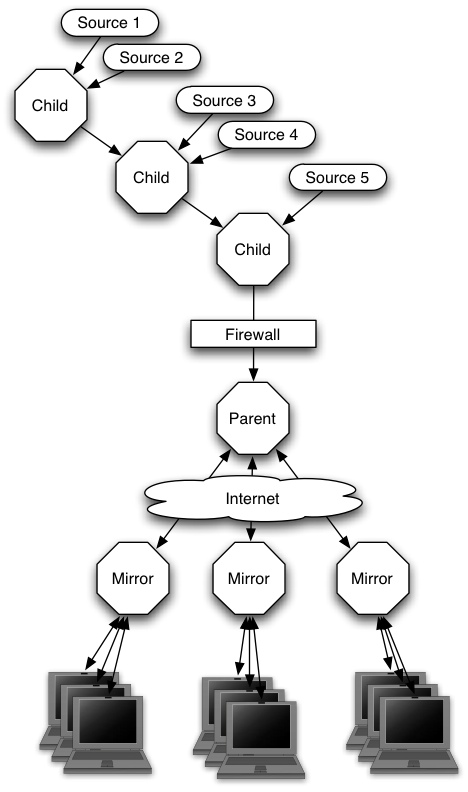
\includegraphics[scale=0.40]{figs/par-child-diagram}} \quad
\subfigure[Parent-child routing as used for experiment.\label{fig:ucla-arch}]{ 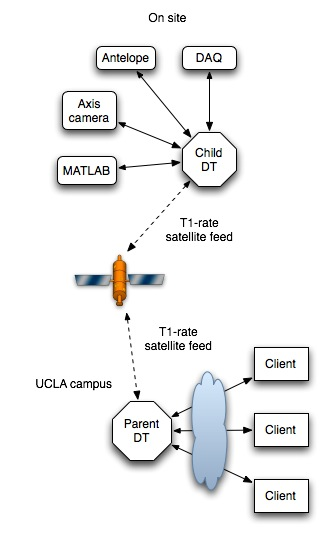
\includegraphics[scale=0.40]{figs/UCLA}}
}
\caption{Observing system models}
\label{fig:rbnb-topo}
\end{center}
\end{figure*}    

Using parent-child, arbitrarily deep routing trees can be constructed, with host-based access control at each vertex/server. This is often used to place a child or children behind a firewall or NAT, with the parent as public. This works because the child initiates the connection to the parent, and will periodically attempt to reconnect if an error occurs.

Other topologies are possible using the mirroring capabilities. RBNB DataTurbine can mirror between servers very easily.
% , and also includes an experimental 'Robust Routing Plugin' which is designed to be tolerant of network errors. 
Mirroring is useful for load balancing, scalability and robustness. It is particularly useful in isolating client load from server load, so that inbound data is not delayed or lost. 
% Another feature that we've not yet utilized is called shortcuts. These are setup via the administrative interface and are equivalent to soft links in a filesystem. Shortcuts can be used to create user-transparent links between servers that have an associated cost metric, allowing an efficiently routed multiserver network for the user.

\emph{Challenge 5 - Support for in-network processing and time synchronization: }
% Time synchronization:
% Time synchronization is important for any distributed system and therefore there is a considerable amount of work available for time synchronization for distributed systems~\cite{lamport-78, lamport-85,mills94}

In-network processing provides opportunity for data fusion, event detection, and QA/QC
across multiple sensor data streams~\cite{madden02tag}. To that end, RBNB provides capabilities for
in-network data buffering and processing. For example, Figure~\ref{fig:routing-arch} shows how data from multiple sources can be processed at multiple levels using tree topology. This provides an opportunity to perform application-specific in-network processing at various stages along the path between a data source and a data sink.

Time synchronization is especially critical in sensor networks for a variety of reasons including sensor data aggregation, power-efficient duty cycling. 
% Data reported by a sensor cannot be interepreted unless the physical context of the reporting sensor such as its location and the timestamp of the reading is known. 
There has been a considerable research on this topic~\cite{elson-02, elson-report-02, karp-03,sichitiu03} mostly in the context of resource-constrained micro-sensor nodes. 

Deployment experience teaches that synchronized computer clocks are an absolute necessity when trying to view, analyze or display data from distributed systems. In particular, clients request data from the RBNB server based on time, so if the clients' clock is off, the data they get back may be missing or nonsensical. As explained in Section~\ref{sec:rbnb-internals}, key to the idea of RBNB is that all data is timestamped.  Timestamps can be explicit (provided by the source), or implicit (automatically provided by the client API or RBNB server). Therefore, time synchronization is absolutely necessary. However, resource constraints were not an issue in any of our deployments, mainly because most of the use of line power or renewable energy source such as solar power. Therefore, we did not focus development on novel time synchronization protocols. In fact, in our deployments we used standard time synchronization protocols developed for resource-rich distributed systems.  More specifically, we used NTP servers and locally-attached GPS clocks, depending on the experiment.


%, in our deployments, we have used a broad range of options for time synchronization ranging from the use of an in-situ GPS receiver to a NTP server.   %local GPS-based NTP server. 
% Microsoft Windows, in its default non-domain installation, corrects the clock once every eight days which causes errors of up to several minutes. It can be quite difficult to explain to a domain scientist that the time on their laptop is why they cannot view data successfully! Open-source NTP clients on all machines is a solution to the problem and should be planned for in any deployment.

\emph{Challenge 6 - Support for Spatial Data and Visualization Services: }
Data from a sensor network is inherently spatial and temporal.  The size and complexity of the planned observatories necessitates visual and map-based services for scientific analysis and system management. Online mapping interfaces provide a convenient user environment for managing sensors, visualizing their characteristics and mapping sensor data vis-�-vis a variety of spatial data layers. 

To that end, a recent addition to the capabilities of the RBNB DataTurbine is Google Earth integration. Via 'plugins', a DataTurbine mechanism for closely coupled data transformation, streamed data is converted into KML format and displayed in Google Earth. For geospatial data such as Earth-observing systems, this provides a visual interface that domain experts find simpler to understand and navigate. It has also proven invaluable for understanding data trends over an area. As GPS-enabling becomes less expensive, uses such as these are increasingly prevalent and we are therefore focussing on metadata standards to make it easier to do.

\emph{Challenge 7 - Coupling sensor data with modeling tools: }
Answering grand science questions depends critically on developing models for understanding processes such as carbon cycling, algal blooms, climate change, water cycling. This understanding is especially challenging due to factors such as multiscale interactions, coupled biological/chemical/physical models~\cite{hamilton-97}, high spatio-temporal variability~\cite{kratz-03}, and non-linear dynamics~\cite{scheffer-01}.  This demands integration of modeling and analysis tools that can use the real-time data streams from the RBNB DataTurbine. To that end, it is possible to meld the rich image and numeric toolkits of Matlab with the real-time data streams from the RBNB DataTurbine. For example, a Matlab program can perform the image processing on video stream that RBNB acquires from networked cameras. With Version 6 and later of Matlab, direct calls to Java are supported from the command line mode of Matlab.  Thus, Matlab uses the native Java RBNB API directly.  Several simple utility M-files are provided as examples along with the open-source version of the RBNB DataTurbine. We want to point 
out that integration with Matlab is just an example of how analysis tools can be integrated with RBNB
DataTurbine. However, modularity and well documented APIs of RBNB can be facilitate integration of
other analysis tools.

A crucial component of research based on data streaming from sensors is that the quality of the data be known. The large volumes of data will require automation of the quality assurance (QA) and quality control (QC) processing.  Modern sensor network QA/QC agents should be able to monitor the sensor operation continuously, spot abnormal data readings, and provide information so that appropriate actions can be taken to mitigate any potential problems. Based on our interaction with collaborating scientists, we feel that integration of Matlab and other statistical packages with RBNB DataTurbine 
can help them perform QA/QC on real-time data streams. Note that, QA/QC can happen at multiple
stages in an observing system and could even be done by exploiting the in-network processing support of RBNB as discussed in Challenge 5.

